%%%%%%%%%%%%%%%%%%%%%%%%%%%%%%%%%%%%%%%%%%%%%%%%%%%%%%%%%%%%%%%%%%%%%%%%%%%%%%%%
%
% Template license:
% CC BY-NC-SA 3.0 (http://creativecommons.org/licenses/by-nc-sa/3.0/)
%
%%%%%%%%%%%%%%%%%%%%%%%%%%%%%%%%%%%%%%%%%%%%%%%%%%%%%%%%%%%%%%%%%%%%%%%%%%%%%%%%

%----------------------------------------------------------------------------------------
%	PACKAGES AND OTHER DOCUMENT CONFIGURATIONS
%----------------------------------------------------------------------------------------

\documentclass[
11pt, % The default document font size, options: 10pt, 11pt, 12pt
%oneside, % Two side (alternating margins) for binding by default, uncomment to switch to one side
%chapterinoneline,% Have the chapter title next to the number in one single line
spanish,
singlespacing, % Single line spacing, alternatives: onehalfspacing or doublespacing
%draft, % Uncomment to enable draft mode (no pictures, no links, overfull hboxes indicated)
%nolistspacing, % If the document is onehalfspacing or doublespacing, uncomment this to set spacing in lists to single
%liststotoc, % Uncomment to add the list of figures/tables/etc to the table of contents
%toctotoc, % Uncomment to add the main table of contents to the table of contents
parskip, % Uncomment to add space between paragraphs
%codirector, % Uncomment to add a codirector to the title page
headsepline, % Uncomment to get a line under the header
]{MastersDoctoralThesis} % The class file specifying the document structure

\usepackage{tikz}
\usetikzlibrary{positioning,shapes,arrows,automata,fit,calc,babel}

%----------------------------------------------------------------------------------------
%	INFORMACIÓN DE LA MEMORIA
%----------------------------------------------------------------------------------------

\thesistitle{Monitoreo ambiental integrado a Enterprise Buildings Integrator de Honeywell} % El títulos de la memoria, se usa en la carátula y se puede usar el cualquier lugar del documento con el comando \ttitle

% Nombre del posgrado, se usa en la carátula y se puede usar el cualquier lugar del documento con el comando \degreename
%\posgrado{Carrera de Especialización en Sistemas Embebidos} 
\posgrado{Carrera de Especialización en Internet de las Cosas} 
%\posgrado{Carrera de Especialización en Intelegencia Artificial}
%\posgrado{Maestría en Sistemas Embebidos} 
%\posgrado{Maestría en Internet de las cosas}

\author{Ing. Gonzalo Nahuel Vaca} % Tu nombre, se usa en la carátula y se puede usar el cualquier lugar del documento con el comando \authorname

\director{Esp. Ing. Pablo Almada (FIUBA-UTN)} % El nombre del director, se usa en la carátula y se puede usar el cualquier lugar del documento con el comando \dirname
%\codirector{Nombre del codirector (pertenencia)} % El nombre del codirector si lo hubiera, se usa en la carátula y se puede usar el cualquier lugar del documento con el comando \codirname.  Para activar este campo se debe descomentar la opción "codirector" en el comando \documentclass, línea 23.

\juradoUNO{Mg. Ing. Christian Yanez Flores (FIUBA)} % Nombre y pertenencia del un jurado se usa en la carátula y se puede usar el cualquier lugar del documento con el comando \jur1name
\juradoDOS{Esp. Ing. Lucas Fabricio Monzón Languasco (FIUBA-UNNE)} % Nombre y pertenencia del un jurado se usa en la carátula y se puede usar el cualquier lugar del documento con el comando \jur2name
\juradoTRES{Esp. Ing. Daniel Marquez (FIUBA-UC)} % Nombre y pertenencia del un jurado se usa en la carátula y se puede usar el cualquier lugar del documento con el comando \jur3name

\ciudad{Ciudad Autónoma de Buenos Aires}
%\ciudad{ciudad de Mendoza}

\fechaINICIO{mayo de 2020}
\fechaFINAL{abril de 2021}


\keywords{Sistemas embebidos, Internet de las Cosas, FIUBA} % Keywords for your thesis, print it elsewhere with \keywordnames


\begin{document}


\frontmatter % Use roman page numbering style (i, ii, iii, iv...) for the pre-content pages

\pagestyle{plain} % Default to the plain heading style until the thesis style is called for the body content


%----------------------------------------------------------------------------------------
%	RESUMEN - ABSTRACT 
%----------------------------------------------------------------------------------------

\begin{abstract}
\addchaptertocentry{\abstractname} % Add the abstract to the table of contents
%
%The Thesis Abstract is written here (and usually kept to just this page). The page is kept centered vertically so can expand into the blank space above the title too\ldots
\centering

Esta memoria describe la implementación de una solución realizada para los  laboratorios Gador, donde se adapta su sistema de automatización de edificios y gestión empresarial marca Honeywell. La finalidad es integrar una red de sensores que utilizan un protocolo de comunicación que este sistema no puede interpretar.

Se logró cumplir con las necesidades de Gador utilizando contenidos y habilidades desarrollados en las asignaturas de esta especialización. Se creó una arquitectura de datos, se implementaron protocolos de comunicaciones, se programaron servidores y se puso en funcionamiento un sistema de despliegue automático y orquestación de la aplicación.

\end{abstract}

%----------------------------------------------------------------------------------------
%	CONTENIDO DE LA MEMORIA  - AGRADECIMIENTOS
%----------------------------------------------------------------------------------------

%\begin{acknowledgements}
%\addchaptertocentry{\acknowledgementname} % Descomentando esta línea se puede agregar los agradecimientos al índice
%\vspace{1.5cm}
%
%Esta sección es para agradecimientos personales y es totalmente \textbf{OPCIONAL}.  
%
%\end{acknowledgements}

%----------------------------------------------------------------------------------------
%	LISTA DE CONTENIDOS/FIGURAS/TABLAS
%----------------------------------------------------------------------------------------

\tableofcontents % Prints the main table of contents

\listoffigures % Prints the list of figures

\listoftables % Prints the list of tables


%----------------------------------------------------------------------------------------
%	CONTENIDO DE LA MEMORIA  - DEDICATORIA
%----------------------------------------------------------------------------------------

\dedicatory{\textbf{Dedicado a la memoria del Ing. Valeriy Omelchenko}}  % escribir acá si se desea una dedicatoria

%----------------------------------------------------------------------------------------
%	CONTENIDO DE LA MEMORIA  - CAPÍTULOS
%----------------------------------------------------------------------------------------

\mainmatter % Begin numeric (1,2,3...) page numbering

\pagestyle{thesis} % Return the page headers back to the "thesis" style

% Incluir los capítulos como archivos separados desde la carpeta Chapters

% Chapter 1

\chapter{Introducción general} % Main chapter title

\label{Chapter1} % For referencing the chapter elsewhere, use \ref{Chapter1} 
\label{IntroGeneral}

%----------------------------------------------------------------------------------------

% Define some commands to keep the formatting separated from the content 
\newcommand{\keyword}[1]{\textbf{#1}}
\newcommand{\tabhead}[1]{\textbf{#1}}
\newcommand{\code}[1]{\texttt{#1}}
\newcommand{\file}[1]{\texttt{\bfseries#1}}
\newcommand{\option}[1]{\texttt{\itshape#1}}
\newcommand{\grados}{$^{\circ}$}

%----------------------------------------------------------------------------------------

%\section{Introducción}

%----------------------------------------------------------------------------------------
El capítulo presenta las necesidades a satisfacer y una introducción técnica breve, con el objetivo de proveer los conceptos necesarios para comprender el resto de la memoria.

\section{Motivación}
\label{ch1Motivacion}

La tendencia tecnológica actual es interconectar los dispositivos a través de la Internet, a tal punto que la cantidad de objetos en el año 2009 superó al número de personas conectadas, y llegado el 2020 la diferencia es de seis veces en favor de las cosas. \citep{ARTICLE:DaveEvans}
Los procesos industriales se ven beneficiados con nuevos métodos de control de inventarios y análisis de mediciones, además es posible gestionar los ambientes productivos para lograr una mayor calidad y comodidad.
Los datos quedan disponibles para ser procesados por modelos de inteligencia artificial, y la información resultante puede ser vista desde cualquier ubicación y en múltiples plataformas. 

% Realidad de la industria local
Las empresas locales están retrasadas en su progreso tecnológico, muchas no incorporaron sistemas electrónicos en sus procesos o productos, es necesario crear un sistema que logre adaptar la tecnología en uso con el fin de incorporarlas a las nuevas prácticas de negocios.
El avance tecnológico modifica el marco normativo de las naciones, para cumplir con los nuevos requerimientos jurídicos, se necesita tener un mínimo de capital.
El retraso tecnológico ya no solo genera una pérdida de competitividad, sino que también impide que las empresas coloquen sus mercancías en otros países, por incumplimiento en normas de calidad o de protección del medio ambiente.
		
% Necesidades de Gador
% Referencia a la página de Gador	
La situación de la industria argentina fue la primera razón que impulsó este trabajo, el siguiente paso fue buscar una empresa que quisiera participar de un proyecto adecuado para el pos-grado, y finalmente se logró un acuerdo con los laboratorios Gador S.A. La misión de la compañía es producir medicamentos para la salud humana, con la mejor calidad disponible, y ponerlos al alcance de la comunidad a precios accesibles. \citep{WEBSITE:Gador}

La empresa tiene la necesidad de acceder al mercado estadounidense y para lograrlo se deben satisfacer los requerimientos del \emph{Code of Federal Regulations - Title 21 - Food and Drugs Chapter - Part 11 (21CFR11)}. La norma establece que los registros de las mediciones ambientales de los depósitos y cuartos productivos, se deben almacenar de forma electrónica, pero se debe demostrar que los registros tienen la misma validez y seguridad que aquellos hechos en papel. \citep{ARTICLE:21cfr11} Esto se traduce en la necesidad de tener un sistema informático que se encuentre aprobado por la \emph{Food and Drug Administration (FDA)}, que es el organismo encargado de controlar los medicamentos y alimentos que ingresan a los Estados Unidos.
Por esa razón Gador tiene comprada una licencia del sistema \emph{Enterprise Buildings Integrator (EBI)} de la marca \emph{Honeywell}, ya que el producto se encuentra aprobado por la FDA. 
Si bien el programa fue adquirido hace varios años, es indispensable que continúe operando aún cuando los protocolos que utiliza son antiguos. Tampoco es económicamente viable reemplazarlo por un producto moderno que esté aprobado por la FDA, se debe lograr un salto tecnológico manteniendo la plataforma que actualmente está operando.

% Perfiles térmicos
Los requerimientos que se deben cumplir en las mediciones ambientales de los depósitos y cuartos productivos, estipulan que los sensores se deben someter a un plan de calibración rutinario y realizarles periódicos estudios de perfiles térmicos.
Un estudio de perfil térmico se logra tomando una serie de mediciones de temperatura en varios puntos de un ambiente, y con estos datos se procede a calcular las coordenadas de los puntos críticos del cuarto. \citep{ARTICLE:Temperature}
Los puntos críticos son aquellos lugares donde la temperatura es la más baja o más alta dentro de la habitación.
Teniendo los puntos críticos identificados, se procede a colocar sensores de temperatura en esos lugares.

% Migración de sensores
Los periódicos estudios de perfiles térmicos, tienen como consecuencia que cada seis meses se deben mover los sensores de temperatura.
La tarea de migrar los dispositivos se vuelve costosa debido a que se encuentran cableados, y además los nuevos recorridos de los cables se deben certificar por el departamento de calidad. El tiempo de migración y de certificación se vería reducido sensiblemente si los equipos fuesen inalámbricos, pero la licencia de EBI que tiene Gador no es compatible con los protocolos de comunicaciones necesarios para lograrlo.

% Arquitectura de la red industrial Gador
Las plantas de producción de la empresa siguen una arquitectura en donde los sensores reportan sus mediciones a unos controladores lógicos programables o PLC por sus siglas en inglés. Esa comunicación se logra a través de cables que los conectan. Los datos que adquieren los PLCs son entregados al sistema EBI utilizando un protocolo de comunicaciones llamado Modbus TCP. 
Este protocolo fue creado en el año 1979 y se diseñó teniendo en mente las limitaciones tecnológicas de la época, sin embargo la licencia de EBI que adquirió Gador solo acepta este formato. El modelo lógico de la arquitectura se puede visualizar en la figura \ref{fig:redGador}, donde se puede ver una estructura del tipo árbol donde todo converge al sistema EBI.
			
\begin{figure}[h]
	\centering
	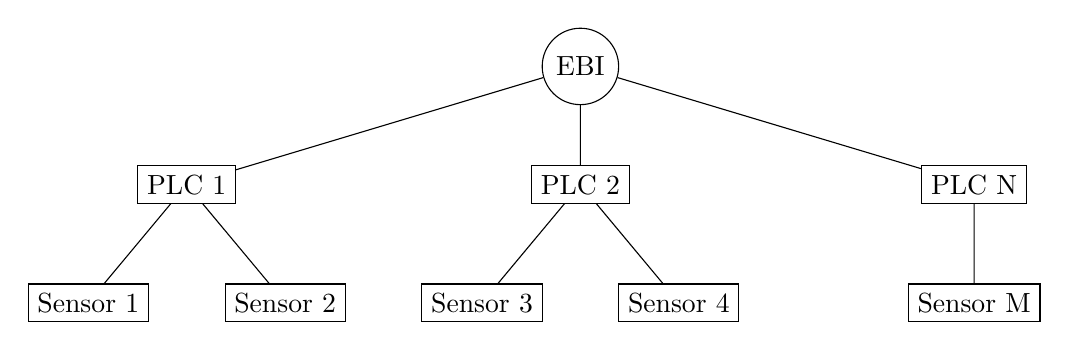
\begin{tikzpicture}[level 1/.style={sibling distance=5cm},
						level 2/.style={sibling distance=2.5cm}]
		\node[circle,draw]{EBI}
			child{
				node[rectangle,draw]{PLC 1}
					child[rectangle,draw]{node[rectangle,draw]{Sensor 1}}
					child[rectangle,draw]{node[rectangle,draw]{Sensor 2}}
				}
			child{
				node[rectangle,draw]{PLC 2}
					child{node[rectangle,draw]{Sensor 3}}
					child{node[rectangle,draw]{Sensor 4}}
				}
			child{
				node[rectangle,draw]{PLC N}
				child{node[rectangle,draw]{Sensor M}}
				}
		;
	\end{tikzpicture}
	\caption{Red industrial Gador.}
	\label{fig:redGador}
\end{figure}


\section{Introducción técnica}
\label{ch1IntroduccionTecnica}

% Presentación modelo de capas IoT
El proyecto realizado presentó una serie de desafíos a resolver, siendo el primero de ellos la variedad de tecnologías involucradas, tanto en la problemática a manipular como en la solución a implementada.
Para introducir orden en la variedad de conocimientos que forman parte del sistema desarrollado, se introduce un modelo de capas de Internet de las cosas (IoT). El modelo tiene la ventaja que separa los temas en categorías relacionadas con la función o servicio que prestan en la solución, lo que facilita su estudio. 

% Enumeración de las capas y una breve descripción de cada una
El modelo de capas seleccionado separa los conocimientos en cinco categorías, las cuales son las capas de negocio, aplicación, procesamiento, red y percepción.
La capa de negocio agrupa todo lo relacionado con las reglas y el control del sistema, esto incluye supervisar el tráfico de información, verificar el estado de los equipos u otorgar permisos a los usuarios para interactuar con el programa.
La capa de aplicación relaciona todas las tecnologías que se encargan de interactuar con el usuario final, es lo que las personas pueden ver como el sistema.
La capa de procesamiento agrupa los conocimientos cuya responsabilidad es almacenar y analizar los datos que se generan.
La capa de red tiene la finalidad de interconectar los dispositivos para permitir el flujo de datos entre todas las partes involucradas.
Finalmente la capa de percepción se refiere a todos los artefactos que manipulan o miden algo que se encuentra en el ambiente, como un sensor o un actuador. Este modelo se encuentra resumido en la tabla \ref{tab:modeloCapas}.

\begin{table}[h]
	\centering
	\caption{\label{tab:modeloCapas}Modelo de capas IoT.}
	\begin{tabular}{c c}
		\toprule
		\textbf{Capa} & \textbf{Función}                         \\
		\midrule
		Negocio       & Establecer reglas y controlar el sistema \\
		Aplicación    & Interactuar con el usuario               \\
		Procesamiento & Almacenar y analizar los datos obtenidos \\
		Red           & Transportar los datos entre dispositivos \\
		Percepción    & Realizar mediciones o acciones en planta \\
		\bottomrule
		\hline
	\end{tabular}
\end{table}

% Capa de negocios
Dependiendo del modelo viabilidad económica de un sistema y de como fue desplegado, la capa de negocio puede tener una funcionalidad contable y calcular los costos de operación.
Esta capa puede ser la encargada de determinar y generar la facturación para cobrarle a los usuarios de la aplicación, como así también, de resolver operaciones de transferencia de dinero.
La interacción en este nivel es con el personal que administra un sistema, se determina que permisos tiene cada usuario para manipular los servicios ofrecidos y se lleva adelante el registro de acciones y eventos relevantes para el normal funcionamiento del programa.

% Capa de aplicación
La experiencia que tiene el usuario al interactuar con la solución pertenece a la capa de aplicación.
Aquí se define como se presenta la interfaz gráfica que utilizan las personas, y es común utilizar un formato de sitio web.
Las páginas webs tienen la ventaja de ser indiferentes de la plataforma que utiliza el operador, solo importa que pueda ejecutar un navegador.
Actualmente, se construyen las interfaces siguiendo un modelo de diseño según el tipo de operación a realizar por el programa, si la solución abarca una interfaz hombre-máquina industrial que debe ser atendida durante toda una jornada laboral, se suele implementar una norma de manejo de situaciones anormales o ASM; si la aplicación es de uso intermitente, se puede usar un esquema de diseño material o \emph{Material Desing} que presenta una experiencia moderna y fluida, como se puede apreciar en la figura \ref{fig:ch1MaterialDesign}.
Para llevar a delante la interfaz seleccionada se utiliza un servidor que tiene como objetivo proveer los componentes gráficos al dispositivo utilizado, una manera de realizarlo es entregando al cliente una \emph{Single Web Application (SWP)}, logrando que el servidor otorgue todo el código necesario para que el dispositivo del usuario genere por si mismo los componentes gráficos a mostrar.
Es importante que el código entregado pueda ser visualizado en múltiples tamaños de pantallas, en la actualidad las personas utilizan ordenadores, tabletas y teléfonos móviles que presentan grandes diferencias en sus dimensiones, cuando una aplicación cumple con este requerimiento se dice que es responsiva.

% poner referencia de la figura en pie de página
% https://material.io/blog/mda-2020-winners
\begin{figure}[h]
	\centering
	\includegraphics[width=\textwidth]{./Figures/ch1MaterialDesign.jpg}
	\caption{Ejemplo de interfaz de diseño material. \citep{WEBSITE:Material}}
	\label{fig:ch1MaterialDesign}
\end{figure}

% Capa de procesamiento
Para alimentar de datos a la interfaz gráfica se necesita de la capa de procesamiento, que entrega el contenido a mostrar en pantalla. La información puede ser almacenada con distintas tecnologías, siendo una de las principales, las bases de datos relacionales.
Este tipo de base de datos se basa en un esquema de tablas que se relacionan entre sí.
Estas tecnologías se las suelen llamar SQL, y son utilizadas principalmente en datos de inventarios y sistemas de transacciones de dinero.
Existe otro grupo de bases de datos que se denominan no relacionales o NoSQL, esta categoría contienen a las bases de datos tipo clave-valor, documental, de columnas y de grafos.

% clave-valor
Las bases de datos clave-valor tratan los datos como una única colección que puede tener campos completamente distintos en cada registro, no existe entonces, ningún tipo de relación entre los miembros de la colección. El uso principal de esta tecnología es gestionar diccionarios dentro de la memoria volátil, ya que se pueden definir tiempos de vida para los datos. La muerte programada de un dato puede ser utilizada para gestionar las sesiones de usuario dentro del programa.

% documental
Almacenar los datos de manera documental significa que se agrupa la información siguiendo un criterio de entidades similares, lo cual no significa que exista una estructura rígida, sino que los datos tienen una naturaleza similar.
La persistencia se logra siguiendo un formato de codificación estandar como \emph{XML}, \emph{YAML} y \emph{JSON}.

% columnas
Las bases de datos orientadas a columnas están pensadas para minimizar el tiempo de búsqueda, principalmente en series temporales.
La organización particular de este tipo de tecnologías es afín a los sistemas de IoT ya que los dispositivos de mediciones suelen generar un gran volumen de datos, que se pueden organizar como series temporales.

% grafos
Una base de datos orientada a grafos presenta la información como nodos que se encuentran relacionados, la diferencia fundamental con los sistemas relacionales es que los nodos no están organizados en tablas, y las relaciones que unen los nodos tienen atributos y no poseen una estructura definida.
Este tipo de tecnología permite utilizar la teoría de grafos y posibilita realizar consultas siguiendo modelos matemáticos que forman parte de esa rama de la ciencia.

% Capa de red
Se dispone de un repertorio de protocolos pertenecientes a la capa de red para lograr que los dispositivos se comuniquen entre si.
Entre los mencionados a lo largo de esta memoria se encuentran el protocolo Modbus, MQTT, HTTP y WebSocket. El manejo de estas tecnologías fue fundamental para lograr que las distintas partes del trabajo interactúen con el exterior.

% Modbus
Modbus es un protocolo que se diseñó teniendo en cuenta su uso para aplicaciones industriales, su prioridad es transmitir los datos manteniendo su integridad aún en ambientes donde el ruido eléctrico es elevado. El protocolo es público y gratuito, lo que provocó que se impusiera en un gran segmento del mercado ya que además es fácil de implementar y requiere poco desarrollo. Los dispositivos de una red Modbus tienen una dirección única y por lo general se asigna un equipo como maestro y el resto como esclavos. La arquitectura descripta presenta varias ventajas, pero la antigüedad del protocolo y su diseño para dispositivos del tipo PLC, hace que no sea adecuado para aplicaciones IoT.

% MQTT
Para interconectar a los dispositivos bajo un esquema de publicación-subscripción se utiliza el protocolo MQTT.
El protocolo está diseñado para conexiones en lugares remotos donde los dispositivos funcionan con un ancho de banda limitado.
El resultado es que los mensajes son pequeños y consumen poca batería de los equipos involucrados, por lo que se usa frecuentemente en los sistemas de IoT.
El tráfico es gestionado por un servidor del tipo broker que decide quienes son los destinatarios de un mensaje en particular, el resto de los dispositivos son clientes del broker.
Si un cliente desea transmitir datos, lo hace realizando una publicación a un determinado \emph{topic} y el broker se encarga de determinar quienes deben recibir la información enviada.
Quienes quieran obtener los datos publicados a un \emph{topic} en particular, se deben suscribir a él ante el broker.
Este al recibir una publicación de un cliente la transmite solo a los clientes que se encuentres subscritos, como se puede ver en el ejemplo de la figura \ref{fig:ch1MqttEjemplo}, donde el cliente 2 no obtiene los datos del sensor porque no se encuentra subscrito.

\begin{figure}[h]
	\centering
	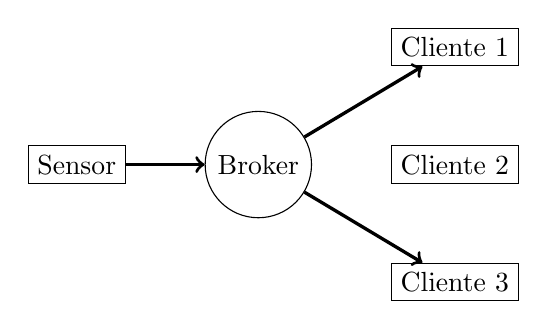
\begin{tikzpicture}
		\tikzstyle{broker} = [circle,draw=black]
		\tikzstyle{publish} = [rectangle,draw=black]
		\tikzstyle{subscribe} = [rectangle,draw=black]
		\tikzstyle{flecha} = [->,very thick]

		\node[publish] (p) {Sensor};
		\node[broker,right=of p] (b) {Broker};
		\node[subscribe, right=of b] (s2)	{Cliente 2};
		\node[subscribe,above=of s2] (s1) {Cliente 1};
		\node[subscribe, below=of s2] (s3) {Cliente 3};

		\draw[flecha] (p) edge (b);
		\draw[flecha] (b) edge (s1);
		\draw[flecha] (b) edge (s3);			
	\end{tikzpicture}
	\caption{Ejemplo de comunicación MQTT.}
	\label{fig:ch1MqttEjemplo}
\end{figure}

% HTTP y Websocket
El protocolo de transferencia de hipertexto (HTTP) está orientado a transacciones y sigue el esquema petición-respuesta entre un cliente y un servidor.
El cliente inicia la comunicación enviando una petición al servidor, este último entrega una respuesta y se cierra el canal.
Existe una variante del protocolo llamada HTTPS que agrega una capa de cifrado para que las comunicaciones sean seguras.

WebSocket es un protocolo similar a HTTP pero con la diferencia que la conexión es bidireccional, esto quiere decir que cuando se logra la conectar al cliente con el servidor, ambos pueden enviar información espontáneamente. Esta cualidad permite realizar transferencias de datos en vivo, con lo que se pueden lograr servicios de \emph{streaming} o \emph{chats}.

% Capa de percepción
Los sensores utilizados en una solución de IoT están incluidos en la capa de percepción, y para que puedan formar parte del sistema se necesita que sean capaces de soportar alguno de los protocolos de comunicaciones mencionados. Dado que el desarrollo de estos dispositivos no formaron parte del proyecto realizado, no se ampliará demasiado en este tema.

% Despliegue de una solución
Teniendo definido los componentes de las capas, se necesita lograr que todas las partes funcionen como una única entidad. Para lograr este objetivo existen tecnologías de despliegue y orquestación, que cumplen la función de interconectar y mantener los servicios para que trabajen en equipo. Tradicionalmente se solían utilizar máquinas virtuales pero actualmente ese enfoque está quedando en desuso en favor de las tecnologías de contenedores. Una máquina virtual acapara parte de una computadora y funciona como un ordenador independiente, mientras que un contenedor funciona como un sistema operativo independiente pero no acapara los recursos de la computadora principal.


\section{Estado del arte}
\label{ch1EstadoDelArte}

% La nube
En la sección \ref{ch1IntroduccionTecnica} se presentó un modelo de capas para analizar las tecnologías.
En esta sección se utiliza el mismo esquema para presentar las técnicas que conforman el estado del arte.
Es importante mencionar el concepto de nube, ya que las soluciones modernas se basan en utilizar este tipo de plataforma.
La nube se refiere a utilizar servicios y servidores provistos por un tercero.
Entre los sistemas más representativos se encuentran \emph{Amazon Web Service (AWS)}, \emph{Google Cloud} y \emph{Azure}.
Estas empresas ofrecen su infraestructura y una serie de facilidades que promueven un rápido desarrollo y despliegue en el mercado.

% Percepción
Los sensores o actuadores que se utilizan corren un firmware específico para el ecosistema utilizado.
Si se decidió utilizar AWS, por ejemplo, lo más probable es que la capa de percepción ejecute \emph{AWS IoT Core} en sus dispositivos.
Este esquema es ampliamente utilizado a nivel \emph{enterprise}, por ejemplo, los laboratorios Bayer utilizan el ecosistema de AWS. \citep{WEBSITE:AWSBayer}

% Transporte
En la capa de transporte, los dispositivos se comunican usualmente utilizando los protocolos \emph{LoRaWAN}, \emph{Sigfox}, \emph{ZigBee} o \emph{Bluetooth}.
La selección del protocolo depende de las distancias a cubrir y de las necesidades energéticas.
Los sensores convergen luego a un punto de agregación.
Desde los puntos de agregación se suelen transmiten los datos al servidor en la nube utilizando el protocolo MQTT.

% Procesamiento
En la capa de procesamiento se utiliza un esquema de datos de alta disponibilidad.
Esto se logra creando réplicas de los datos en distintos servidores.
Una de las réplicas se configura como maestro y el resto como esclavos.
El servidor maestro es quien se comunica con el exterior de la réplica y retransmite los nuevos datos a los esclavos.
Si un servidor maestro sufre un problema, uno de los esclavos se convierte en el nuevo maestro y se mantiene a la réplica funcionando sin interrupciones.

Los datos pueden ser divididos en \emph{shards}, esto se hace para dividir la base de datos según la aplicación.
Un ejemplo es separar los datos por región geográfica, de esta manera los clientes de una región en particular pueden tener los servidores con los datos que suelen utilizar cerca de ellos.
Para que los \emph{shards} funcionen como una única base de datos, se dispone de un servidor \emph{router} que es la interfaz con el exterior.
El \emph{router} recibe las consultas o ingresos de nuevos datos y se encarga de utilizar el \emph{shard} correspondiente.
La configuración de este sistema se maneja desde un grupo de servidores destinados para tal fin.
Suelen conformar una réplica donde solo se almacenan los datos de configuración.
Esta arquitectura de alta disponibilidad se la conoce como granja de datos, se la puede construir con mongoDB \citep{WEBSITE:mongodbSharding} y se encuentra visualizada en la figura \ref{fig:ch1DatosAltaDisponibilidad}.

\begin{figure}[h]
	\centering
	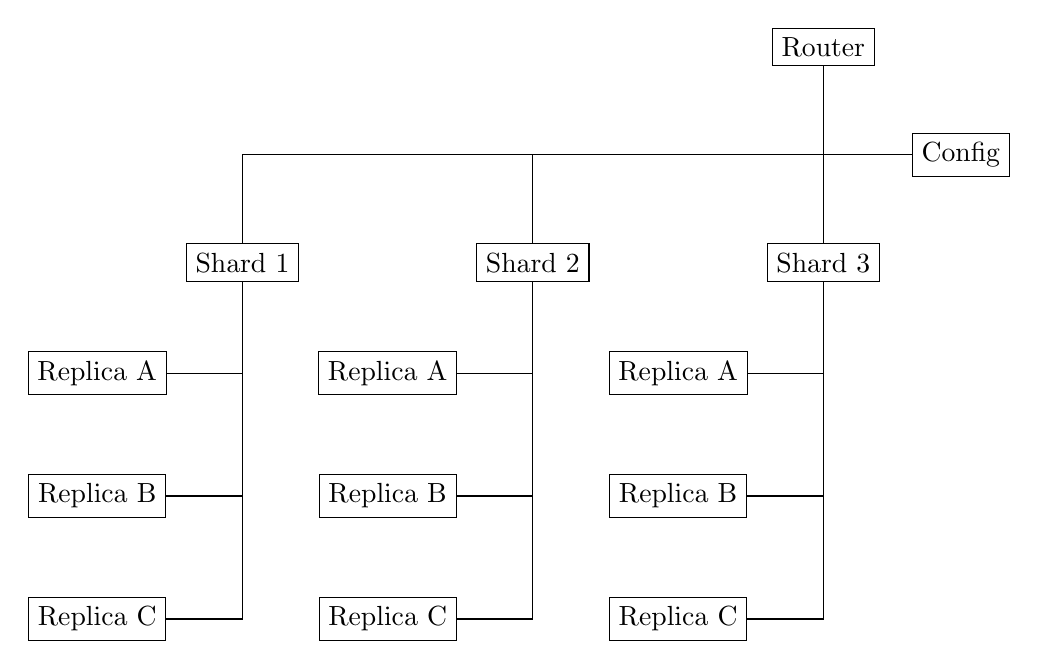
\begin{tikzpicture}		
		\tikzstyle{block} = [rectangle,draw=black]
				
		\node[block] (r) {Router};
		
		\node[below=of r] (aux) {};
		\node[block,right=of aux] (c) {Config};
		
		\node[block,below=of aux] (s3) {Shard 3};
		\node[left=of s3] (aux1) {};
		\node[block,left=of aux1] (s2) {Shard 2};
		\node[left=of s2] (aux2) {};
		\node[block,left=of aux2] (s1) {Shard 1};
		\node[left=of s1] (aux3) {};
		
		\node[block,below=of aux3] (ra1) {Replica A};
		\node[block,below=of ra1] (ra2) {Replica B};
		\node[block,below=of ra2] (ra3) {Replica C};
		
		\node[block,below=of aux2] (rb1) {Replica A};
		\node[block,below=of rb1] (rb2) {Replica B};
		\node[block,below=of rb2] (rb3) {Replica C};
		
		\node[block,below=of aux1] (rc1) {Replica A};
		\node[block,below=of rc1] (rc2) {Replica B};
		\node[block,below=of rc2] (rc3) {Replica C};
				
		\draw (r)--(s3);
		\draw (s1)|-(c);
		\draw (s2)|-(c);
		\draw (s3)|-(aux);
		\draw (c)--(aux);
		
		\draw (ra1)-|(s1);
		\draw (ra2)-|(s1);
		\draw (ra3)-|(s1);	
		
		\draw (rb1)-|(s2);
		\draw (rb2)-|(s2);
		\draw (rb3)-|(s2);
		
		\draw (rc1)-|(s3);
		\draw (rc2)-|(s3);
		\draw (rc3)-|(s3);
	\end{tikzpicture}
	\caption{Arquitectura de datos de alta disponibilidad.}
	\label{fig:ch1DatosAltaDisponibilidad}
\end{figure}

% Aplicación
La capa de aplicación se suele diseñar rápidamente con un framework dedicado a la construcción de interfaces gráficas.
Uno de los más utilizados es Angular, desarrollado por la empresa Google.
El estilo gráfico de diseño material presentado en la sección \ref{ch1IntroduccionTecnica} es la más utilizada.
Las plataformas de nube ofrecen sus propios sistemas para diseñar la aplicación sin necesidad de escribir demasiado código, pero estas facilidades generan erogaciones adicionales.

% Negocio
La plataforma de nube presenta una capa de negocios donde se puede controlar el tráfico del sistema en ejecución.
Desde allí se puede ver la facturación estimada o el consumo de crédito para mantener en funcionamiento el proyecto.
En esta capa se pueden cambiar las variables de entorno del sistema y se pueden controlar el estado de los componentes.
Es posible montar servicios que corran programas como \emph{Checkmk} o \emph{Grafana} para visualizar el estado de los dispositivos en campo. O se puede optar por usar los servicios que ofrezca la empresa de nube.

% Orquestación y despliegue
La tecnología que se suele utilizar para orquestar toda la solución es Kubernetes, ya que además de automatizar el despliegue, también permite ajustar la escala.
Ajustar la escala se refiere a la capacidad de crear una réplica de un servicio cuando uno de ellos está trabajando cerca de su límite de procesamiento.
Es un sistema basado en contenedores y crea un \emph{clúster} a partir de una plantilla donde se definen las reglas de escalamiento.

\section{Objetivos y alcance}
\label{objetivos}

% Objetivos
El objetivo principal que cumplió este proyecto fue demostrarle al cliente el potencial de las nuevas tecnologías y la posibilidad de integrarlas a sus actuales sistemas.
Se propuso crear una prueba de concepto para evaluar la viabilidad de futuros proyectos.
La creación de un sistema que pueda unir equipos que utilizan Modbus con aquellos que usan MQTT, es de relevancia en general para la industria local.
Otro objetivo importante fue la de utilizar las técnicas adquiridas durante la cursada de la especialización.
Con la finalidad de sementar los conocimientos a través de la práctica.

% Alcance
El proyecto se limitó a desarrollar el software a desplegar en un servidor que fue nombrado Nodos.
Esto significa que no se contempló el desarrollo del hardware, en particular los sensores y los puntos de agregación.
E esquema del servidor en la red de Gador puede ser visualizado en la figura \ref{fig:esquemaProyecto}.
El servidor puede comunicarse con EBI de la misma manera que lo logra un PLC.
Además tiene la capacidad de utilizar el protocolo MQTT para conectarse directamente con los sensores o a través de puntos de agregación.


\begin{figure}[h]
	\centering
	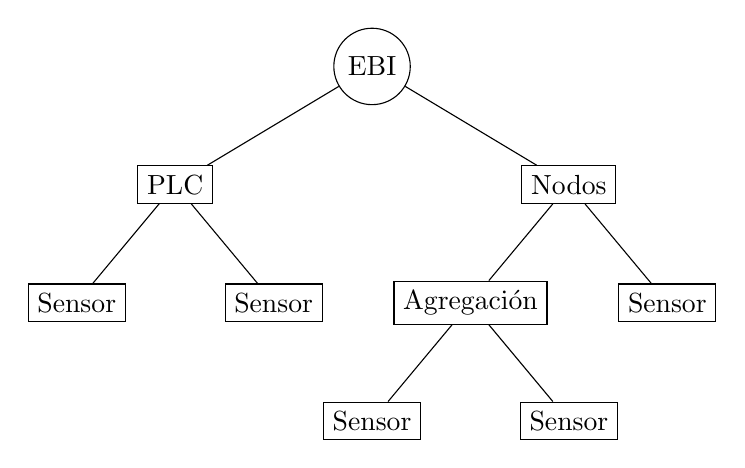
\begin{tikzpicture}[level 1/.style={sibling distance=5cm},
						level 2/.style={sibling distance=2.5cm}]
		\node[circle,draw]{EBI}
			child{
				node[rectangle,draw]{PLC}
					child[rectangle,draw]{node[rectangle,draw]{Sensor}}
					child[rectangle,draw]{node[rectangle,draw]{Sensor}}
				}
			child{
				node[rectangle,draw]{Nodos}
					child{
						node[rectangle,draw]{Agregación}
							child[rectangle,draw]{node[rectangle,draw]{Sensor}}
							child[rectangle,draw]{node[rectangle,draw]{Sensor}}
					}
					child{node[rectangle,draw]{Sensor}}
				}
		;
	\end{tikzpicture}
	\caption{Red industrial Gador.}
	\label{fig:esquemaProyecto}
\end{figure}

% Requerimientos
Cuando se tuvo definidos los objetivos y el alcance del proyecto, se inició un proceso de negociación con el cliente.
Se buscó determinar cuales eran sus necesidades y sus temores respecto del proyecto.
Las conversaciones con el cliente dieron como resultado la siguiente lista de requerimientos:

\begin{itemize}
	\item Debe integrarse a la infraestructura de Gador S.A. sin generar conflictos en otros sistemas.
	\item Debe crear tramas en el formato \emph{Enterprise Buildings Integrator} y enviarlas al servidor.
	\item Debe interpretar eventuales mensajes del servidor \emph{Honeywell}.
	\item Debe interpretar los mensajes de los sensores.
	\item Debe poder cambiar la frecuencia de lectura de mediciones.
	\item Debe poseer la capacidad de gestionar los ingresos de usuarios de forma segura.
	\item Debe permitir que por lo menos cinco usuarios accedan al sistema simultáneamente.
	\item Debe presentar una interfaz donde se monitoree el estado de los sensores
	\item Debe permitir elegir un sensor en particular para editarlo.
	\item Debe poseer un módulo de gestión de usuarios.
	\item Debe ser compatible con ordenadores de escritorio y smartphones.
	\item Las contraseñas no persistirán como texto plano.
	\item Debe persistir todas las modificaciones realizadas a la configuración de los sensores.
	\item Debe persistir las mediciones obtenidas.
\end{itemize}
\chapter{Introducción específica} % Main chapter title

\label{Chapter2}

%----------------------------------------------------------------------------------------
%	SECTION 1
%----------------------------------------------------------------------------------------
Este capítulo trata sobre los recursos tecnológicos utilizados en el trabajo que fueron desarrollados por terceros.

% Descripción de las plataformas tecnológicas que sostienen al trabajo
\section{Tecnologías utilizadas}

% docker
\emph{Docker} es un software que permite el uso y creación de contenedores de Linux.
Un contenedor es una unidad que empaqueta el código de un programa junto con sus dependencias.
Para crear un contenedor, \emph{Docker} se vale de el concepto de imagen.
Las imágenes son entidades aisladas que corren como contenedores durante el tiempo de ejecución sobre el motor de \emph{Docker}.
Los contenedores son entonces, una abstracción de la capa de aplicación de los sistemas Linux, como se puede visualizar en la figura \ref{fig:ch2WhatContainer}.
Varios contenedores pueden correr en el mismo ordenador como procesos aislados en el espacio de usuario.
La principal diferencia con las máquinas virtuales, es que estas son una abstracción del hardware del ordenador, transformando una única computadora en varios servidores.
Los contenedores en cambio, utilizan el kernel del sistema operativo del ordenador físico, no se abstrae un kernel, solo el espacio de aplicación o usuario.

% docker files
\emph{Docker} puede ser utilizado para construir imágenes definidas por el usuario.
Un \emph{Dockerfile} es un documento de texto que contiene todos los comandos que un usuario utilizaría para ensamblar una imagen.
El programador puede crear automáticamente una serie de comandos en sucesión al ejecutar un único comando sobre el \emph{Dockerfile}. 

% docker compose
\emph{Docker Compose}, según se define en su documentación \citep{WEBSITE:WhatDockerCompose}, es una herramienta para definir y correr aplicaciones de \emph{Docker} de múltiples contenedores.
Permite utilizar un archivo \emph{YAML} para configurar los servicios de la aplicación.
Luego, se puede crear y comenzar todos los servicios de la configuración utilizando un único comando.

\begin{figure}[h]
	\centering
	\includegraphics[width=\textwidth]{./Figures/ch2DockerContainer.png}
	\caption{Arquitectura de \emph{Docker}. \citep{WEBSITE:WhatContainer}}
	\label{fig:ch2WhatContainer}
\end{figure}

% nodejs
\emph{Nodejs} es un servidor asincrónico y orientado a eventos que ejecuta JavaScript.
Estas cualidades son una ventaja frente a las aplicaciones de concurrencia de múltiples hilos en el sistema operativo.
Ya que no se utilizan candados, no existe la posibilidad de bloquear el servidor.
Dado que fue diseñado para construir aplicaciones de red escalables, se eligió para formar parte del trabajo.

% python
\emph{Python} es un lenguaje de programación interpretado que tiene una gran cantidad de bibliotecas a disposición.
Muchas bibliotecas fueron útiles para desarrollar algunos servicios pequeños del proyecto.
Se utilizó para acelerar la creación de las partes más livianas del sistema.

% mosquitto
\emph{Eclipse Mosquitto} es un \emph{broker MQTT}.
Es liviano y puede ser ejecutado en ordenadores monoplaca.
Permite ser configurado con varios niveles de calidad de servicio, se pueden agregar usuarios con distintos permisos y es posible utilizar una capa de seguridad en los mensajes.
Uno de sus atractivos es la serie de programas utilitarios que incluye el proyecto y se integran en la terminal del sistema operativo.
Estas aplicaciones permiten realizar publicaciones y subscripciones para realizar pruebas, además se pueden crear contraseñas encriptadas para los usuarios.

% mongodb
"\emph{MongoDB} es una base de datos distribuida, basada en documentos y de uso general diseñada para desarrolladores de aplicaciones modernas y para la era de la nube". \citep{WEBSITE:MongoHome}
Se decidió utilizar esta tecnología para la capa de procesamiento debido a la afinidad que posee para realizar aplicaciones \emph{IoT}.
Además es la base de datos documental más utilizada actualmente \citep{WEBSITE:DBRanking} y se evaluó como aspecto relevante, ganar experiencia con esta tecnología.

% redis
	
% Descripción de las dependencias del trabajo
\section{Bibliotecas y paquetes de terceros}

% Angular & Angular Material

% express & cors

% mqtt & ws

% mongoose

% bcrypt & jsonwebtoken

% chai & mocha

% pyModbusTCP

% paho MQTT

% oitc/modbus-server

% Descripción del sistema marca Honeywell que funciona en planta.
\section{Sistema propietario del cliente} 
\chapter{Diseño e implementación} % Main chapter title

\label{Chapter3} % Change X to a consecutive number; for referencing this chapter elsewhere, use \ref{ChapterX}

\definecolor{mygreen}{rgb}{0,0.6,0}
\definecolor{mygray}{rgb}{0.5,0.5,0.5}
\definecolor{mymauve}{rgb}{0.58,0,0.82}

%%%%%%%%%%%%%%%%%%%%%%%%%%%%%%%%%%%%%%%%%%%%%%%%%%%%%%%%%%%%%%%%%%%%%%%%%%%%%
% parámetros para configurar el formato del código en los entornos lstlisting
%%%%%%%%%%%%%%%%%%%%%%%%%%%%%%%%%%%%%%%%%%%%%%%%%%%%%%%%%%%%%%%%%%%%%%%%%%%%%
\lstset{ %
  backgroundcolor=\color{white},   % choose the background color; you must add \usepackage{color} or \usepackage{xcolor}
  basicstyle=\footnotesize,        % the size of the fonts that are used for the code
  breakatwhitespace=false,         % sets if automatic breaks should only happen at whitespace
  breaklines=true,                 % sets automatic line breaking
  captionpos=b,                    % sets the caption-position to bottom
  commentstyle=\color{mygreen},    % comment style
  deletekeywords={...},            % if you want to delete keywords from the given language
  %escapeinside={\%*}{*)},          % if you want to add LaTeX within your code
  %extendedchars=true,              % lets you use non-ASCII characters; for 8-bits encodings only, does not work with UTF-8
  %frame=single,	                % adds a frame around the code
  keepspaces=true,                 % keeps spaces in text, useful for keeping indentation of code (possibly needs columns=flexible)
  keywordstyle=\color{blue},       % keyword style
  language=[ANSI]C,                % the language of the code
  %otherkeywords={*,...},           % if you want to add more keywords to the set
  numbers=left,                    % where to put the line-numbers; possible values are (none, left, right)
  numbersep=5pt,                   % how far the line-numbers are from the code
  numberstyle=\tiny\color{mygray}, % the style that is used for the line-numbers
  rulecolor=\color{black},         % if not set, the frame-color may be changed on line-breaks within not-black text (e.g. comments (green here))
  showspaces=false,                % show spaces everywhere adding particular underscores; it overrides 'showstringspaces'
  showstringspaces=false,          % underline spaces within strings only
  showtabs=false,                  % show tabs within strings adding particular underscores
  stepnumber=1,                    % the step between two line-numbers. If it's 1, each line will be numbered
  stringstyle=\color{mymauve},     % string literal style
  tabsize=2,	                   % sets default tabsize to 2 spaces
  title=\lstname,                  % show the filename of files included with \lstinputlisting; also try caption instead of title
  morecomment=[s]{/*}{*/}
}


%----------------------------------------------------------------------------------------
%	SECTION 1
%----------------------------------------------------------------------------------------
En este capítulo se detallan las tareas realizadas durante el trabajo.
Se explica como se crearon los servicios y como se interconectaron para lograr una orquestación.
% Explicación sobre el funcionamiento y la creación de la arquitectura y del código que automáticamente despliega la aplicación en un servidor
\section{Arquitectura y orquestación}
Esta sección trata sobre la conexión entre los servicios del trabajo y su despliegue automático.

Para planificar la orquestación se analizaron los servicios que debían ser accesibles desde entidades externas al servidor.
En la figura \ref{fig:ch3EsquemaTrabajo} se pueden observar las conexiones lógicas entre los contenedores.
Destacadas en color rojo, se encuentran las entidades externas que interactúan con el servidor Nodos.
Las interconexiones se simplificaron al crear una capa de puente de red que corre sobre el mismo \emph{Daemon} de Docker.
El resultado es que cada contenedor pasa a tener una dirección ip dentro del entorno.
La creación de esta red se logró con el el código \ref{cod:dcNetwork}.

\begin{figure}[h]
	\centering
	\includegraphics[width=\textwidth]{./Figures/ch3EsquemaTrabajo.png}
	\caption{Esquema de conexión de los servicios.}
	\label{fig:ch3EsquemaTrabajo}
\end{figure}

\begin{lstlisting}[label=cod:dcNetwork,caption=Red de interconexión Docker Compose.]
networks: 
	iot:
		driver: bridge
\end{lstlisting}

El servicio modbus-server se comunica al exterior utilizando el puerto 502.
El puerto pertenece a la lista de protocolos bien conocidos o puertos de sistema.
Esta condición hace posible que existan problemas con los permisos que el usuario tiene dentro del sistema operativo.
Como se puede observar en el código \ref{cod:dcModbusServer}, se conectó el puerto 502 del sistema operativo con el 5020 dentro de la red de Docker.
En general, es una buena práctica que los puertos internos de la red no sean puertos de sistema para no generar conflictos de permisos y conectarlos a puertos de protocolos según sea necesario.
Para evitar usar direcciones ip en el código de los servicios se utilizó el parámetro hostname para utilizar el servicio de sistema de nombres de dominio (DNS) que corre dentro del \emph{Daemon} de Docker.

\begin{lstlisting}[label=cod:dcModbusServer,caption=Orquestación del servidor Modbus.]
modbus-server:
	image: oitc/modbus-server
	container_name: modbus-server
	hostname: modbus-server
	restart: always
	ports:
		- '502:5020'
	expose: 
    	- '5020'
	networks: 
		- iot
\end{lstlisting}

El servicio Mosquitto se configuró con tres volúmenes que conectan al contenedor con archivos no efímeros que persisten la información necesaria para que el contenedor muestre un comportamiento correcto.
Como se puede apreciar en el código \ref{cod:dcMosquitto}, se encuentran los archivos de configuración de usuarios y de lista de control de acceso (acl).
Con esta configuración se evita que dispositivos anónimos puedan utilizar el broker y que además solo puedan utilizar los \emph{topics} designados.
Además los distintos usuarios tienen diferentes permisos según el \emph{topic}.
De esta manera se logra una mayor confiabilidad y seguridad en el manejo de los mensajes.

\begin{lstlisting}[label=cod:dcMosquitto,caption=Orquestación del broker Mosquitto.]
mosquitto:
	image: eclipse-mosquitto
	container_name: mosquitto
	hostname: mosquitto
	restart: always
	volumes: 
		- ./mosquitto/mosquitto.conf:/mosquitto/config/mosquitto.conf
		- ./mosquitto/users.txt:/mosquitto/config/users.txt
		- ./mosquitto/acl.txt:/mosquitto/config/acl.txt
	expose: 
		- '1883'
		- '9001'
	ports: 
		- '1883:1883'
		- '9001:9001'
	networks: 
		- iot
\end{lstlisting}

El servicio \emph{Holding Registers Validator} (hrv) tiene la particularidad de depender de otros servicios, como se puede ver en el cógigo \ref{cod:dcHRV}.
El contenedor no puede ser creado hasta que los servicios listados como dependencias se encuentren activos.
Esto se hace de esta manera para evitar que el contenedor genere excepciones y se reinicie varias veces durante el despliegue se la solución.
Además no es posible saber si el comportamiento final del contenedor puede quedar indefinido.
Es importante mencionar que este servicio no tiene salida al exterior y no queda visible por la falta de campos \emph{ports}.

La imagen para construir el contenedor no existe y debe ser creada al momento del despliegue.
Para lograrlo se utiliza el campo \emph{build}, en donde se especifica la ruta al Dockerfile que contiene la receta.
La imagen queda guardada con el nombre vaca/hrv, de esta manera, no es necesario volver a construirla si se decide reiniciar la solución.

\begin{lstlisting}[label=cod:dcHRV,caption=Orquestación del servicio hrv.]
hrv:
	build: ./holdingRegistersValidator/
	image: vaca/hrv
	container_name: hrv
	hostname: hrv
	restart: always
	expose: 
		- '1883'
		- '5020'
	depends_on: 
		- 'mosquitto'
		- 'mongo'
		- 'modbus-server'
	networks: 
		- iot
\end{lstlisting}

El Dockerfile que fabrica la imagen puede verse en el código \ref{cod:dfHRV}.
Este código es común para todos los Dockerfiles que construyen imágenes para los servicios realizados en Python.
Se utiliza Alpine Linux como imagen base y se genera el usuario y grupo \emph{pythonuser}.
El usuario es quien corra el servicio dentro del contenedor y se define un comando a ejecutar al momento de crearlo.
Quedan definidos en este archivo cuales son puertos que se pueden usar para la red puente.

\begin{lstlisting}[label=cod:dfHRV,caption=Dockerfile del servicio hrv.]
FROM python:3.8-alpine
LABEL maintainer="Gonzalo Nahuel Vaca <vacagonzalo@gmail.com>"
RUN addgroup -g 1000 -S pythonuser && \
	adduser -u 1000 -S pythonuser -G pythonuser && \
	mkdir -p /app && \
	pip3 install pyModbusTCP && \
	pip3 install paho-mqtt && \
	pip3 install pymongo
ADD --chown=root:root app/* /app/
USER pythonuser
EXPOSE 1883 27017 5020/tcp
CMD [ "python", "-u", "/app/service.py" ]
\end{lstlisting}

El servicio MongoDB no tiene salida al exterior del servidor, su configuración se puede ver en el código \ref{cod:dcMongo}.
La configuración tiene la particularidad de introducir un comando a la hora de crear el contenedor.
Se le indica al motor de MongoDB que puerto debe escurchar.
Además se crea un volumen donde figuran una serie de archivos que pueblan la base de datos con información para construir una maqueta.
Esta maqueta fue utilizada para realizar la demostración al cliente.
Los archivos son devices.js, measurements.js, seed.js y users.js.
El archivo devices.js crea una serie de dispositivos ficticios.
El archivo measurements.js inserta una serie de mediciones que provienen de los dispositivos ficticios creados por devices.js.
El script users.js genera una serie de usuarios con distintos permisos.
Con el fin de probar la capacidad de autentificar las sesiones.
Finalmente seed.js es quién carga todos los datos en MongoDB, según se puede ver en el código \ref{cod:dcSeed}.
Las mediciones fueron cargadas múltiples veces para generar un volumen de datos que sirviera para realizar pruebas.

\begin{lstlisting}[label=cod:dcMongo,caption=Orquestación de MongoDB.]
mongo:
	image: mongo
	container_name: mongo
	hostname: mongo
	command: mongod --bind_ip_all --port 27017
	expose: 
		- '27017'
	volumes: 
		- ./mongodb/scripts:/scripts
	networks:
		- iot
\end{lstlisting}

\begin{lstlisting}[label=cod:dcSeed,caption=Seed de la base de datos.]
use gador;
load("scripts/devices.js")
load("scripts/users.js")
load("scripts/measurements.js")
load("scripts/measurements.js")
load("scripts/measurements.js")
load("scripts/measurements.js")
load("scripts/measurements.js")
load("scripts/measurements.js")
load("scripts/measurements.js")
load("scripts/measurements.js")
load("scripts/measurements.js")
\end{lstlisting}

El servicio Persistence Validator (pv), está definido en el código \ref{cod:dcPV}.
Se puede observar que la imagen no existe y debe ser construida.
Como el servicio fue realizado en Python, el Dockerfile necesario para construir la imagen es prácticamente idéntico al visto en el código \ref{cod:dfHRV}.

\begin{lstlisting}[label=cod:dcPV,caption=Orquestación del servicio pv.]
	pv:
		build: ./persistenceValidator
		image: vaca/pv
		container_name: pv
		hostname: pv
		restart: always
	expose: 
		- '1883'
		- '27017'
	depends_on: 
		- 'mosquitto'
		- 'mongo'
	networks: 
		- iot
\end{lstlisting}

Para orquestar el servicio backend se utilizó el puerto 8080 del ordenador.
La razón es que se tiene una comunicación con una entidad externa, el usuario.
La imagen para crear el contenedor debe ser construida y para tal fin se usó el Dockerfile que se puede observar en el código \ref{cod:dfBackend}.

\begin{lstlisting}[label=cod:dcBackend,caption=Orquestación del servicio Backend.]
backend:
	build: ./backend
	image: vaca/backend
	container_name: backend
	hostname: backend
	expose: 
		- '1883'
		- '6379'
		- '27017'
	ports: 
		- '8080:8080'
	depends_on:
		- 'mosquitto' 
		- 'mongo'
		- 'redis'
	networks: 
		- iot
\end{lstlisting}

El Dockerfile parte de la imagen oficial de Nodejs y copia los archivos de dependencias dentro del contenedor auxiliar.
Con este archivo se descargan las bibliotecas necesarias.
Luego se copia el código fuente de la aplicación y finalmente se configura la inicialización del servidor Nodejs como comando por defecto.

\begin{lstlisting}[label=cod:dfBackend,caption=Dockerfile del servicio Backend.]
FROM node
LABEL maintainer="Gonzalo Nahuel Vaca <vacagonzalo@gmail.com>"
WORKDIR /usr/src/app
COPY package*.json ./
RUN npm install
COPY . .
EXPOSE 1883 6379 8080 27017
CMD ["node", "./src/app.js"]
\end{lstlisting}

El servicio Calibrator es una aplicación de Nodejs y fue orquestada de manera similar al servicio Backend.
Su configuración se puede observar en el código \ref{cod:dcCalibrator}.
El Dockerfile necesario para crear su imagen es prácticamente idéntico al mostrado en el código \ref{cod:dfBackend}.

\begin{lstlisting}[label=cod:dcCalibrator,caption=Orquestación del servicio Calibrator.]
calibrator:
	build: ./calibrator
	image: vaca/calibrator
	container_name: calibrator
	hostname: calibrator
	expose: 
		- '1883'
		- '9999'
	ports:
		- '9999:9999'
	depends_on: 
		- 'mosquitto'
	networks: 
		- iot
\end{lstlisting}

El servicio Redis fue creado a partir de la imagen oficial de Redis que se encuentra disponible en Dockerhub. \citep{contrib:redis}
Como no tiene exposición al exterior del servidor, no se necesitó realizar ninguna configuración adicional.
Es importante aclarar que si bien se puede aplicar una capa de seguridad, no es aconsejable exponer a Redis a la Internet.
La orquestación se puede ver en el código \ref{cod:dcRedis}.

\begin{lstlisting}[label=cod:dcRedis,caption=Orquestación del servicio Redis.]
redis:
	image: redis
	container_name: redis
	hostname: redis
	expose:
		- '6379'
	networks: 
		- iot
\end{lstlisting}

El último servicio es el Frontend que fue orquestado como se puede observar en el código \ref{cod:dcFrontend}.
Su imagen se crea usando el código fuente de la aplicación y un Dockerfile al momento de orquestar la solución.
La construcción de esta imagen es la más sofisticada de todo el trabajo, como se puede ver en el código \ref{cod:dfFrontend}.

\begin{lstlisting}[label=cod:dcFrontend,caption=Orquestación del servicio Frontend.]
frontend:
	build: ./frontend/
	image: vaca/frontend
	container_name: frontend
	hostname: frontend
	restart: always
	ports: 
		- '80:80'
\end{lstlisting}

El Dockerfile se divide en dos grandes etapas.
La primer parte es crear un contenedor auxiliar a partir de la imagen oficial de Nodejs y llamarla \emph{builder}.
Este contenedor temporal copia dentro suyo el código fuente del servicio e instala todas las dependencias.
Entre las dependencias instaladas se encuentra el framework de Angular.
Se utiliza el framework para compilar el código fuente de TypeScript y se obtienen archivos en JavaScript, que son ejecutables por un navegador.
La segunda parte del proceso es crear un contenedor a partir de la imagen oficial de Nginx, que es un servidor web.
Se transfieren los archivos compilados por el contenedor auxiliar hacia el contenedor de Nginx y se destruye el auxiliar.
Finalmente se transforma el contenedor de Nginx con los archivos compilados en una imagen.

\begin{lstlisting}[label=cod:dfFrontend,caption=Dockerfile del servicio Frontend.]
FROM node as builder
WORKDIR /src/app
COPY . ./
RUN npm install
RUN npm run ng build  --prod
FROM nginx
COPY --from=builder /src/app/dist/frontend /usr/share/nginx/html
\end{lstlisting}

Teniendo definido los Dockerfiles y el archivo docker-compose.yml se puede utilizar un guión escrito en Bash que lanza la aplicación.
Como se puede observar en el código \ref{cod:bashStart}.

Cuando se desea eliminar todo rastro del sistema del ordenador.
Se puede utilizar el código \ref{cod:bashClean}.

Los únicos requisitos para iniciar la aplicación es tener un ordenador que tenga Docker y Docker Compose instalados.
No se necesita tener ninguna de las herramientas de desarrollo dentro del ambiente de producción.
De esta manera se logró una solución altamente portable y agnóstica de la arquitectura del hardware.

\begin{lstlisting}[label=cod:bashStart,caption=Guión de inicialización.]
#!/bin/bash
chmod +x clean.sh
docker-compose up -d
printf "Waiting 10 seconds for internal connections to be made"
sleep 10
docker-compose exec mongo sh -c "mongo < /scripts/seed.js"
printf "checking collections"
docker-compose exec mongo sh -c "mongo < /scripts/seed.test.js"
\end{lstlisting}

\begin{lstlisting}[label=cod:bashClean,caption=Guión de limpieza.]
#!/bin/bash
docker-compose down
docker rmi vaca/backend
docker rmi vaca/hrv
docker rmi vaca/pv
docker rmi vaca/auth-api
docker rmi vaca/calibrator
docker rmi vaca/frontend
clear
\end{lstlisting}

% \newpage

% Explicación sobre el funcionamiento y la creación de los servicios que interactuan con dispositivos
% Diagrama de flujo que explique la interacción del sistema con los dispositivos.
\section{Servicios orientados a dispositivos}

% mosquitto
Mosquitto fue configurado siguiendo su documentación para lograr el máximo nivel de seguridad que no incluyera certificados \emph{SSH}.
Se decidió no utilizar certificados ya que no figuraban en los requerimientos y el broker no se encuentra expuesto a la Internet.
Además uno de los motivos del trabajo es simplificar la interacción con los sensores.
Agregar la tarea de controlar y renovar los certificados iba en contra del objetivo inicial.
La configuración puede ser observada en el código \ref{cod:mosquittoConfig}.

\begin{lstlisting}[label=cod:mosquittoConfig,caption=Archivo mosquitto.conf]
allow_anonymous false
password_file /mosquitto/config/users.txt
acl_file /mosquitto/config/acl.txt
\end{lstlisting}

Se creó una configuración de usuarios que tiene en su interior dos usuarios.
El primer usuario se denominó docker y su contraseña es container.
El segundo usuario se nombró device y su contraseña es thing.
Las contraseñas se guardaron encriptadas utilizando la herramienta \emph{mosquitto\_passwd}.
El usuario docker se utiliza para que los contenedores se comuniquen con el broker, mientras que device se asigna a los sensores en campo.
Las diferencias entre contenedores y dispositivos se configuran en el archivo de acl, como se visualiza en el código \ref{cod:mosquittoAcl}.
El topic cmnd se utiliza para los mensajes que alteran la configuración de los dispositivos.
El topic data tiene la finalidad de llevar las mediciones tomadas por los sensores y hacerlas persistir en la base de datos.
Finalmente el topic live tiene la función de llevar las mediciones que se realizan durante las calibraciones.

\begin{lstlisting}[label=cod:mosquittoAcl,caption=Lista de control de acceso]
user docker
topic readwrite cmnd/#
topic read data/#

user device
topic readwrite cmnd/#
topic write data/#
topic write live/#
\end{lstlisting}

% holding register validator
El servicio Holding Register Validator (HRV) tiene la misión de determinar que mediciones se deben escribir en una posición de memoria del servidor Modbus.
Para cumplir con esa función, HRV se subscribe al topic data y recibe todos los reportes de los sensores.
Luego determina si las mediciones recibidas pertenecen a la lista de dispositivos que figuran en la base de datos y si corresponde escribir una posición de memoria.
Finalmente escribe una posición de memoria del servidor según corresponda.
Las funciones de cada paso fueron extraídas y se presentan en el código \ref{cod:HRVpython}, escritas en Python.

\begin{lstlisting}[label=cod:HRVpython,caption=Funciones principales del servicio HRV]
# MQTT
def onMessage(client, userdata, msg):
    data = msg.payload.decode().split(",")
    addr = getAddr(data[0])
    if addr != -1:
        val = int(data[1])
        write_slave(addr, val)
        
# DATABASE
def getAddr(id):
    global devices
    d = devices.find_one({"tag": id})
    if d is None:
        return -1
    if 'modbus' in d:
        return int(d['modbus'])
    return -1

# MODBUS
def write_slave(addr, value):
    global master
    if master.write_single_register(addr, value):
        print('writing successful')
    else:
        print('writing error')
\end{lstlisting}

% persistance validator
El servicio Persistence Validator (PV) tiene la función de recibir las mediciones de los sensores y decidir si deben persistir en la base de datos.
Para tal fin se encuentra subscrito al topic data.
Cuando recibe una medición, verifica que provenga de un sensor válido en la base de datos.
Si se cumpla esta condición se procede a impactar en la colección Readings en MongoDB.
El servicio fue escrito en Python.
Se extrajeron las funciones principales y se las pueden ver en el código \ref{cod:PVpython}.

\begin{lstlisting}[label=cod:PVpython,caption=Funciones principales del servicio PV]
# DATABASE
def insertReading(id, value, unit):
    post = {
        "date": datetime.datetime.utcnow(),
        "tag": id,
        "val": value,
        "unit": unit
    }
    global measurements
    measurements.insert_one(post)

def isValidId(id):
    global devices
    d = devices.find_one({'tag': id})
    return (d is not None)
    
# MQTT
def onMessage(client, userdata, msg):
    unit = msg.topic.split("/")[1][0]
    data = msg.payload.decode().split(",")
    insertReading(data[0], data[1], unit)    
\end{lstlisting}
	
% Explicación sobre el funcionamiento y la creación de los servicios que interactuan con el usuario
% Imágenes del frontend 2 o 3 máx.
\section{Servicios orientados a usuarios}

% calibrator
El servicio Calibrator es un servidor WebSocket.
Tiene la finalidad de entablar una conexión con el navegador del usuario para transmitirle mediciones en vivo.

\begin{lstlisting}[label=cod:Calibrator,caption=Archivo principal del servicio Calibrator]
const mqtt = require('./services/broker');
mqtt.subscribe('live');
const express = require('express');
const cors = require('cors');
const app = express();
app.use(cors());

const server = require('http').createServer(app);

const PORT = process.env.PORT || 9999;
const WebSocket = require('ws');

const wss = new WebSocket.Server({ server });

wss.on('connection', (ws) => {
    ws.on('message', (data) => {
        wss.clients.forEach((client) => {
            client.send(data);
        });
    });
});

mqtt.on('message', (topic, payload) => {
    wss.clients.forEach(client => {
        let data = `${payload}`;
        client.send(data);
    });
});

server.listen(PORT, () => { console.log(`running on: ${PORT}`) }); 
\end{lstlisting}


% backend

% frontend

% Chapter Template

\chapter{Ensayos y resultados} % Main chapter title

\label{Chapter4} % Change X to a consecutive number; for referencing this chapter elsewhere, use \ref{ChapterX}

%----------------------------------------------------------------------------------------
%	SECTION 1
%----------------------------------------------------------------------------------------

Este capítulo tiene la finalidad de explicar el proceso de aceptación del trabajo y como se determinó que los requerimientos se cumplieron. Además se expone la metodología utilizada para validar el código a medida que se fue escribiendo.

\section{Recursos utilizados}

Para desarrollar el trabajo y realizar pruebas se utilizaron una serie de equipos que se detallan a continuación:

\begin{itemize}
	\item Ordenador portátil Banghó
	\item Ordenador monoplaca Raspberry Pi 4 B
	\item Módulo Nodemcu Esp32 Wi-Fi
	\item Smartphone LG K20 Aurora Black
	\item Router Sagemcom F@ST 3890 v2 TLC
\end{itemize}

Los detalles del ordenador portátil son:
\begin{itemize}
	\item Sistema operativo: Ubuntu 20.04 focal
	\item Kernel: x68\_64 Linux 5.4.0-67-generic
	\item Shell: bash
	\item Resolución: 2732x768
	\item Entorno de escritorio: GNOME 3.36.5
	\item CPU: Intel Core i7-4710MQ @ 8x 3.5GHz
	\item GPU: Intel Corporation 4th Gen Core Processor Integrated Graphics Controller (rev 06)
	\item RAM: 11891MiB
\end{itemize}

Se utilizaron además una serie de programas para hacer el desarrollo y las pruebas y se los enumera a continuación:

\begin{itemize}
	\item Visual Studio Code versión 1.54.3
	\item Navegador Chromium versión 89.0.4389.90 (Build oficial) snap (64 bits)
	\item Terminal de Gnome versión 3.36.2
	\item Postman versión 8.0.7
	\item Wireshark versión 3.2.3
	\item Nmap versión 7.80
	\item Mosquitto versión 1.6.9
\end{itemize}

% Explicación del proceso de decición para determinar cuando debí realizar scripts. Descripción de las scripts creados y su valides
\section{Guiones y comandos}
% necesidad de realizar mocks
En el capítulo \ref{Chapter3} se detalló el trabajo realizado, como funcionan todas sus partes y la interdependencia que existe entre ellas. Antes de llegar a tener un sistema completo y funcionando se tuvieron partes incompletas y servicios inexistentes. Esta situación demandó crear una serie de guiones y comandos que pudieran recrear de forma limitada alguna de las funcionalidades de las dependencias de cada componente.

\subsection{Base de datos}

Varios de los servicios necesitaron tener acceso a una conexión de base de datos en MongoDB durante su desarrollo.
Para crear una instancia efímera del motor se utilizó un guión de bash que se puede ver en el código \ref{cod:ch3GuionDB}.
Se puede observar que se utilizó docker para esa etapa del trabajo.
El código se escribió para facilitar variaciones en la configuración y se designó una carpeta para almacenar una serie de archivos en JavaScript que cumplieron la función de poblar con datos a MongoDB.

\begin{lstlisting}[language=bash,label=cod:ch3GuionDB,caption=Guión de base de datos.]
#!/bin/bash
IMAGE_NAME=mongo
CONTAINER_NAME=mongo
CONTAINER_PORT=27017
CONTAINER_DIRECTORY=/scripts
MACHINE_PORT=27017
MACHINE_DIRECTORY=$PWD/mockDB

docker run \
--rm \
--name $CONTAINER_NAME \
-p $MACHINE_PORT:$CONTAINER_PORT \
-v $MACHINE_DIRECTORY:$CONTAINER_DIRECTORY \
-d \
$IMAGE_NAME

sleep 5
docker exec $CONTAINER_NAME sh -c "mongo < /scripts/mockData.js"
\end{lstlisting}

\subsection{Mosquitto}

Los servicios que necesitaron de un broker MQTT para validar su desarrollo se valieron de un guión de bash.
Ese guión, que se puede ver en el código \ref{cod:ch3GuionMosquitto}, se encargó de proveer un broker completamente promiscuo y sin ninguna medida de seguridad.
La razón para generar esta configuración fue eliminar cualquier tipo de falla producto de las medidas de seguridad y que cualquier comportamiento no deseado se debiera al código escrito para cada servicio en particular.

\begin{lstlisting}[language=bash,label=cod:ch3GuionMosquitto,caption=Guión de Mosquitto.]
#!/bin/bash
IMAGE_NAME=eclipse-mosquitto
CONTAINER_NAME=mosquitto
CONTAINER_PORT=1883
MACHINE_PORT=1883

docker run \
--rm \
--name $CONTAINER_NAME \
-p $MACHINE_PORT:$CONTAINER_PORT \
-d \
$IMAGE_NAME
\end{lstlisting}

Se utilizaron los servicios que provee Mosquitto para realizar publicaciones y subscripciones desde la terminal del ordenador portátil y el ordenador monoplaca.
Los comandos se pueden ver de forma genérica en el código \ref{cod:ch3ComandosMosquitto}.

\begin{lstlisting}[language=bash,label=cod:ch3ComandosMosquitto,caption=Comandos de Mosquitto.]
mosquitto_sub -h 'localhost' -u 'docker' -P 'container' -t 'data/#'
mosquitto_pub -h 'localhost' -u 'device' -P 'thing' -t 'data' -m 'edu-ciaa,25'
\end{lstlisting}

\subsection{Redis}

Los componentes del sistema que utilizaron un mecanismo de identificación de clientes usaron Redis para lograrlo.
Por ese motivo se creó un guión de bash que creara un contenedor de Redis con la configuración por defecto.
El código \ref{} muestra las instrucciones necesarias para lograr el objetivo.
Se puede ver en su última línea que se creó un token de prueba para verificar la conexión con el servicio.

\begin{lstlisting}[language=bash,label=cod:ch3GuionRedis,caption=Guión de Redis.]
#!/bin/bash
IMAGE_NAME=redis
CONTAINER_NAME=redis
CONTAINER_PORT=6379
MACHINE_PORT=6379

docker run \
--rm \
--name $CONTAINER_NAME \
-p $MACHINE_PORT:$CONTAINER_PORT \
-d \
$IMAGE_NAME

sleep 5
docker exec redis sh -c "redis-cli SET xxxx.yyyy.zzzz 3"
\end{lstlisting}

\subsection{Nodejs}
Se necesitó crear un ambiente de desarrollo y pruebas para podes escribir el código de los servicios basados en Nodejs.
Esto se logró al construir los componentes que se detallan a continuación:
\begin{itemize}
	\item Archivo de variables de entorno
	\item Archivo de configuración del framework de pruebas Mocha
	\item Creación de guiones en el archivo de paquetes de Nodejs
\end{itemize}



% Explicación de como se implementó TDD en algunos servicios y como se hicieron pruebas unitarias en otras
\section{Pruebas unitarias}
% introducción. Inicio con TDD, abandono de TDD por incremento exponencial en la complejidad de las pruebas.

% Explicación del proceso de decición para determinar cuando debí realizar simulaciones. Descripción de las simulaciones creadas y su valides
\section{Simulaciones}

% Recepción del cliente, sus comentarios y modificaciones realizadas para satisfacerlo
\section{Pruebas del cliente}
 
% Chapter Template

\chapter{Conclusiones} % Main chapter title

\label{Chapter5} % Change X to a consecutive number; for referencing this chapter elsewhere, use \ref{ChapterX}


%----------------------------------------------------------------------------------------

%----------------------------------------------------------------------------------------
%	SECTION 1
%----------------------------------------------------------------------------------------

Párrafo introductorio del capítulo.

% Valor agregado al cliente y mi aprendizaje
\section{Resultados obtenidos}

% Siguientes pasos para implementar el trabajo dentro del ambiente productivo de Gador
\section{Trabajo futuro} 

%----------------------------------------------------------------------------------------
%	CONTENIDO DE LA MEMORIA  - APÉNDICES
%----------------------------------------------------------------------------------------

\appendix % indicativo para indicarle a LaTeX los siguientes "capítulos" son apéndices

% Incluir los apéndices de la memoria como archivos separadas desde la carpeta Appendices
% Descomentar las líneas a medida que se escriben los apéndices

%\include{Appendices/AppendixA}
%\include{Appendices/AppendixB}
%\include{Appendices/AppendixC}

%----------------------------------------------------------------------------------------
%	BIBLIOGRAPHY
%----------------------------------------------------------------------------------------

\Urlmuskip=0mu plus 1mu\relax
\raggedright
\printbibliography[heading=bibintoc]

%----------------------------------------------------------------------------------------

\end{document}  
